\section{Neural Cellular Automata}
\label{methods:NCA}
%%%% --- NCA allgemein --- %%%%
Finding an appropriate update rule is often a particular challenge when modeling CAs \cite{Gilpin:2019:IntroduceNCA}. In NCAs, this update rule is learned using a Neural Network (NN). A Neural Cellular Automaton (NCA) is, therefore, a simple (i.e., small) Neural Network. In image processing, the neighborhood of the CA is usually the pixel grid of the input image. Since the update rule is based only on the "direct" neighbors, the NN in an NCA is limited to using only tiny (e.g., 3x3) filter kernels. These architectural choices make the model very small regarding the number of parameters. In addition, unlike other NNs, NCAs do not pass the input through the model just once to generate the output. Instead, the output is fed back into the model for a fixed number of time steps ("inference steps"). In terms of a CA, we let the model update the state (neighborhood) for a fixed number of iterations until we observe the image state. Then, the loss is computed and backpropagated through the model as in any other NN. 

In addition, NCAs also use additional channels, i.e., a hidden state that is many times larger than the input. This hidden state and the input image form the hidden input and output of NCAs, which are used only by the model itself. This allows the model to spread information over the entire image, even if it takes several time steps. The intermediate states are overwritten at each step, i.e., they are not stored, and only a layer the size of the input image is used for the final output. The hidden state is not used for loss calculation.


%%%% --- Models --- %%%%
\label{methods:NCA:Models}
We used two different NCAs for training. The Backbone-NCA and the Med-NCA, as shown in \autoref{fig:NCA_Models}. The Med-NCA is built from two backbone NCAs. Both models are designed for medical image segmentation and were developed by \cite{kalkhof:2023:medNCA}. Although they can be used with different numbers of inference steps and channels, we have consistently used 64 inference steps and 16 channels, which are zero-seeded. Only 15 channels can be used by the model because the first channel is overwritten with the original input image after each inference step. The standard Med-NCA configuration uses 32 channels but provides only 0.01 more performance on Dice, while the 16-channel variant requires 2.5 times fewer parameters. The Backbone NCA is about 0.033 weaker on Dice than the Med NCA, although this also depends significantly on the training set \cite{kalkhof:2023:medNCA}.

Another difference between the NCAs we used and most other NNs is that they use randomness, e.g., during inference. In each inference step of the model, only a random portion of the computed output is returned to the model in the next inference step. That way, the model can continue to compute only a portion of the previous output in the next iteration. The output is randomly masked with $p=0.5$. This is similar to other NCA approaches in image processing \cite{mordvintsev:2020:growingNCA, sandler:2020:imageSegNCA}. The goal behind the randomness is to simulate asynchronous execution. Both models use kernels of size $3\times3$. Overall, tiny but robust models can be trained this way. 


%%%% --- Backbone-NCA --- %%%%
\subsection{Backbone-NCA}
The Backbone-NCA is build with a simple architecture, as can be seen in \autoref{fig:NCA_Models}. The Backbone NCA is only the one on the right. However, it is a powerful segmentation NCA. According to the ablation study by \cite{kalkhof:2023:medNCA}, it is only slightly weaker than the med-NCA on the hippocampus dataset we also used. Because of its simple architecture and good performance, we decided to explore using this NCA and this dataset first and then see if any results could be replicated on the Med-NCA and other datasets.

The backbone NCA consists of 2 conv2d layers, which are limited to a kernel size of $3\times3$ and have an input and output depth corresponding to the channels, i.e., 16 in our experiments. These two layers are arranged in parallel, and their output is merged with the input via two linear layers with intermediate Relu. This model block is run through in each inference step. After each inference step, the generated output is merged with the original input again, forming the input for the next inference step. After all (in our case 64) inference steps, the loss is computed using the ground truth labels and propagated back using the PyTorch \cite{paszke:2019:pytorch} backward function.


%%%% --- Med-NCA --- %%%%
\subsection{Med-NCA}  
\label{methods:NCA:Med-NCA}
The Med-NCA is the more powerful segmentation NCA we use. It is build of two Backbone-NCAs and uses additional up- and downscaling and patching, as can be seen in \autoref{fig:NCA_Models}. For this reason, we decided to test the transferability to another model with this NCA after the results could be achieved with the Backbone NCA. We also used it to test the transferability to the more difficult prostate dataset. 

It is based on 2 Backbone-NCAs connected in series. The first Backbone-NCA works with low-resolution inputs. After the 64 inference steps of the first NCA, the output is scaled up again and sent to the second NCA together with the input image. The second NCA continues to work directly on the output of the first NCA at a higher resolution. The second NCA trains on patches to reduce the VRAM. This is no longer necessary after training. The loss is only calculated on the final output and fed back through both models after the second model has also been executed with 64 inference steps.

\begin{figure}[h!]
    \centering
    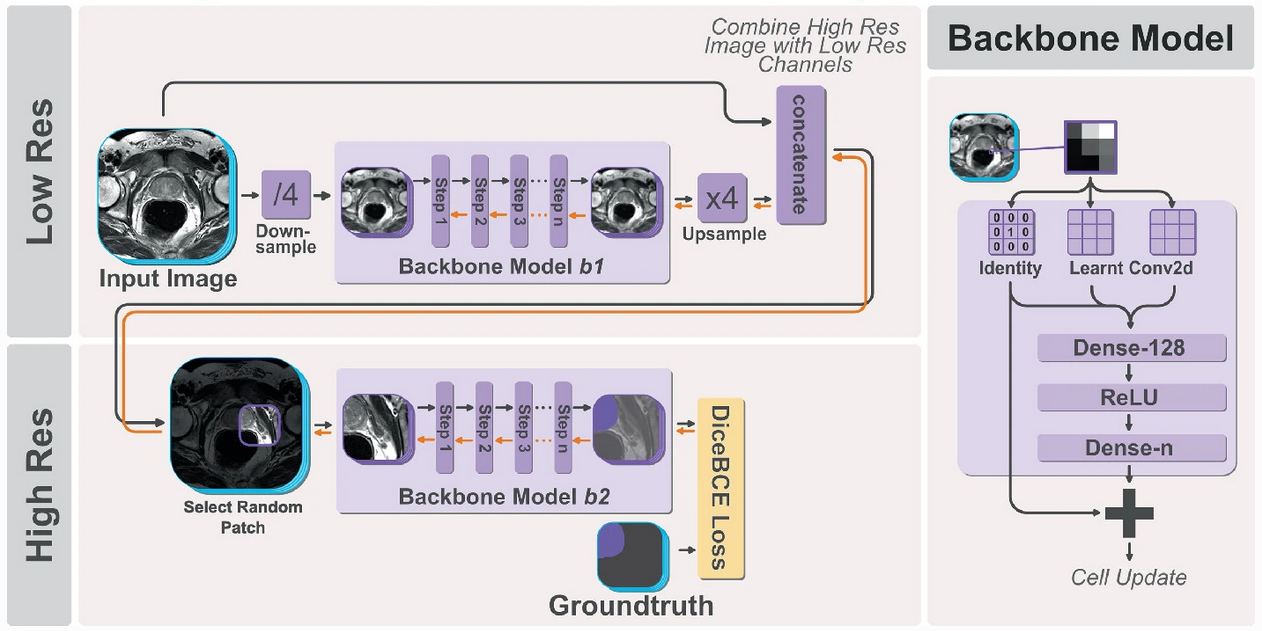
\includegraphics[width=\linewidth]{Graphics/MedNCA_2D.png}
    \caption{The NCAs we used. On the right: The Backbone-NCA, a simple architecture. Whole image: The Med-NCA, using 2 Backbone-NCAs. One training on the whole image, but with low resolution, and one training on high-resolution patches. Patching is not needed after training but reduces VRAM usage. When using the Backbone-NCA alone, we also used the DiceBCE loss. Models and image from \cite{kalkhof:2023:medNCA}.}
    \label{fig:NCA_Models}
\end{figure}

%%%% --- DiceBce Loss --- %%%%
\subsection{DiceBCE Loss}
\label{DiceBCE-Loss}
Both the Backbone-NCA and the Med-NCA use the DiceBCE as the loss. The DiceBCE consists of two parts: the complement of the S{\o}renson-Dice coefficient (Dice or Dice-Loss) and the Binary Cross Entropy (BCE). The DiceBCE is simply the addition of the Dice-Loss and the BCE (\ref{eq:DiceBCE_1}). We use 'Dice' inconsistently for both the complement (i.e. as loss) and the score itself, although it should be apparent from the context what is meant. In particular, only the complement is used as the loss, and only the S{\o}renson-Dice coefficient itself is used as the score for testing, and we never form the complement of the complement or anything like that.

The Dice is the harmonic mean of precision and recall (\ref{eq:DiceBCE_2}), which can be transformed to (\ref{eq:DiceBCE_3}), where TP, FP, and FN stand for True Positive, False Positive, and False Negative, respectively. Overall, the Dice also emphasizes true positives over false positives. For an image volume, where $x_n$ is a prediction $\in(0,1)$ and $y_n$ is a ground truth label $\in(0,1)$ and $n$ is the size of the vectors, i.e., the size of the image volume is $n$. The dice can then be rewritten as (\ref{eq:DiceBCE_4}), where a smoothing factor is added to avoid zero derivatives.

The BCE weights the prediction and rejection ($x_n$ and $(1-x_n)$) logarithmic before multiplying them by the ground truth and then adding them. This element weighting is done for operations on vectors, such as image volumes, where we then reduce by the mean (\ref{eq:DiceBCE_5}). The BCE also maximizes the logarithmic weighted correct predictions of the model and thus minimizes the logarithmic weighted incorrect predictions. The DiceBCE also maximizes the logarithmic weighted correct predictions of the model with a shift towards the true positives.

We used the binary cross entropy function from PyTorch \cite{paszke:2019:pytorch} with reduction for the BCE.
This version of the DiceBCE was used for both the Backbone-NCA and the Med-NCA and proved very effective. Therefore, we used it as a reference in our experiments, and as a starting point for other loss functions we tested.

\begin{align}
    \mathrm{DiceBCE}    &:= 1 - \mathrm{Dice} + \mathrm{BCE},           \label{eq:DiceBCE_1}\\[10pt]
    \mathrm{Dice}       &:= 2 \cdot \frac{\mathrm{precision} \cdot \mathrm{recall}}
                                            {\mathrm{precision} + \mathrm{recall}}          \label{eq:DiceBCE_2}\\[10pt]
                        &= \quad \frac{2 \cdot \mathrm{TP}}
                                   {2 \cdot \mathrm{TP} + \mathrm{FP} + \mathrm{FN}}        \label{eq:DiceBCE_3}\\[10pt]
                        &= \quad \frac{2 \cdot {\sum(x_n \cdot y_n)} +1}
                                   {\sum(x_n) + \sum(y_n) +1}                               \label{eq:DiceBCE_4}\\[10pt]
   \mathrm{BCE}         &:= \mathrm{mean}\ ( -[y_n \cdot \log x_n + (1-y_n) \cdot \log (1-x_n)])        \label{eq:DiceBCE_5}
\end{align}